%==========================================================
% CHAPTER 3: Pirmykštė funkcija ir integralas (A kursas)
%==========================================================
\chapter{Pirmykštė funkcija ir integralas (A kursas)}

\section{Pirmykštės funkcijos sąvoka}

Iki šiol mokėmės \textbf{diferencijuoti} -- turėdami funkciją $f(x)$, radome jos išvestinę $f'(x)$.
Integralų skaičiavimas sprendžia \emph{atvirkštinį} uždavinį: turime funkciją $f(x)$ ir
ieškome tokios funkcijos $F(x)$, kurios išvestinė yra lygi $f(x)$.

\begin{definition}[Pirmykštė funkcija]
Funkcija $F(x)$ vadinama funkcijos $f(x)$ \textbf{pirmykštė funkcija} intervale $(a;\,b)$,
jeigu kiekviename šio intervalo taške teisinga lygybė
\[
    F'(x) = f(x).
\]
\end{definition}

\begin{example}
Funkcija $F(x) = x^3$ yra funkcijos $f(x) = 3x^2$ pirmykštė funkcija, nes
\[
    \bigl(x^3\bigr)' = 3x^2.
\]
Taip pat $F(x) = x^3 + 5$ yra tos pačios funkcijos $f(x)=3x^2$ pirmykštė funkcija, nes
\[
    \bigl(x^3 + 5\bigr)' = 3x^2.
\]
\end{example}

Pastebime, kad pirmykštė funkcija \emph{nėra vienintelė}: pridėjus bet kokią konstantą $C \in \mathbb{R}$,
gaunama kita tos pačios funkcijos pirmykštė funkcija.

\subsection*{Pirmykščių funkcijų egzistavimas ir bendroji forma}

\begin{theorem}[Pirmykščių funkcijų skirtumas]
Jei $F_1(x)$ ir $F_2(x)$ yra funkcijos $f(x)$ pirmykštės funkcijos tame pačiame intervale, tai
\[
    F_1(x) - F_2(x) = C,
\]
kur $C$ yra konstanta.
\end{theorem}

\begin{proof}
Tarkime, kad $F_1'(x) = f(x)$ ir $F_2'(x) = f(x)$. Nagrinėkime funkciją $H(x) = F_1(x) - F_2(x)$.
Tuomet
\[
    H'(x) = F_1'(x) - F_2'(x) = f(x) - f(x) = 0.
\]
Kadangi $H'(x)=0$ visame intervale, tai $H(x) = C = \mathrm{const}$, t.\,y.\
$F_1(x) - F_2(x) = C$.
\end{proof}

Iš šios teoremos išplaukia svarbi išvada: jei žinoma \emph{viena} funkcijos $f(x)$ pirmykštė funkcija
$F(x)$, tai \textbf{visos} pirmykštės funkcijos yra pavidalo
\[
    F(x) + C, \quad C \in \mathbb{R}.
\]

\begin{remark}
Konstanta $C$ vadinama \textbf{integravimo konstanta}. Ji parodo, kad kiekviena funkcija $f(x)$
turi \emph{begalę} pirmykščių funkcijų -- jos visos skiriasi tik vertikaliu grafiko pastūmimu.
\end{remark}

\subsection*{Geometrinė prasmė}

Geometriškai visos funkcijos $f(x)$ pirmykštės funkcijos $F(x)+C$ yra kreivių šeima
$y = F(x) + C$: kiekviena kreivė gaunama iš $y = F(x)$ ją pastumiant aukštyn arba žemyn per
$C$ vienetų. Kiekvieno taško $x_0$ kiekvienoje šių kreivių liestinės nuolydis yra
$f(x_0)$.

\begin{center}
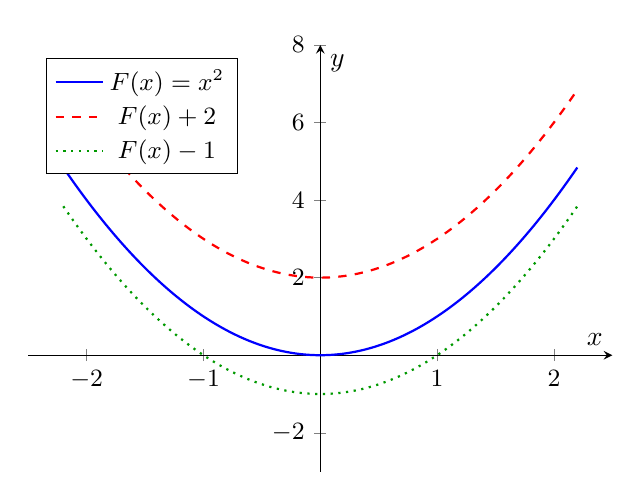
\begin{tikzpicture}
\begin{axis}[
    width=9cm, height=7cm,
    axis lines=center,
    xlabel={$x$}, ylabel={$y$},
    xmin=-2.5, xmax=2.5,
    ymin=-3, ymax=8,
    samples=200,
    domain=-2.2:2.2,
    legend pos=north west,
    legend style={font=\small},
    tick label style={font=\small},
]
\addplot[blue, thick] {x^2};
\addlegendentry{$F(x)=x^2$}

\addplot[red, thick, dashed] {x^2 + 2};
\addlegendentry{$F(x)+2$}

\addplot[green!60!black, thick, dotted] {x^2 - 1};
\addlegendentry{$F(x)-1$}
\end{axis}
\end{tikzpicture}
\end{center}

Grafike matome tris funkcijos $f(x)=2x$ pirmykštes funkcijas: $x^2$, $x^2+2$ ir $x^2-1$.
Jos visos yra vienodo pavidalo parabolės, tik pastumtos skirtingai.

\subsection*{Pirmykštės funkcijos radimas iš pradinės sąlygos}

Dažnai uždaviniuose reikia rasti \emph{konkrečią} pirmykštę funkciją, naudojant pradinę sąlygą --
žinomą funkcijos reikšmę viename taške.

\begin{example}
Raskite funkcijos $f(x) = 2x$ pirmykštę funkciją $F(x)$, jei $F(1) = 3$.

\textbf{Sprendimas.} Žinome, kad $F(x) = x^2 + C$. Iš sąlygos $F(1)=3$:
\[
    1^2 + C = 3 \implies C = 2.
\]
Todėl $F(x) = x^2 + 2$.
\end{example}

\subsection*{Fizikinė prasmė}

Pirmykštė funkcija turi aiškią fizikinę interpretaciją:
\begin{itemize}
    \item Jei $v(t)$ yra kūno \textbf{greitis} laiko momentu $t$, tai jo \textbf{kelias} (nueitas atstumas)
          $s(t)$ yra funkcijos $v(t)$ pirmykštė funkcija, nes $s'(t)=v(t)$.
    \item Jei $a(t)$ yra kūno \textbf{pagreitis}, tai greitis $v(t)$ yra funkcijos $a(t)$
          pirmykštė funkcija, nes $v'(t)=a(t)$.
\end{itemize}

\begin{exercise}
Automobilio greitis duodamas formule $v(t) = 6t^2 + 4t$ (m/s). Raskite nuvažiuoto kelio
funkciją $s(t)$, jei $s(0) = 0$.
\end{exercise}

\begin{example}[Pratimo sprendimas]
Ieškome $s(t)$, kur $s'(t)=v(t)=6t^2+4t$. Vadinasi:
\[
    s(t) = 2t^3 + 2t^2 + C.
\]
Iš sąlygos $s(0)=0$: $C=0$. Atsakymas: $s(t) = 2t^3 + 2t^2$.
\end{example}

\subsection*{Ryšys su neapibrėžtiniu integralu}

Visų funkcijos $f(x)$ pirmykščių funkcijų aibė vadinama \textbf{neapibrėžtiniu integralu}
ir žymima
\[
    \int f(x)\,\mathrm{d}x = F(x) + C,
\]
kur $F'(x) = f(x)$ ir $C \in \mathbb{R}$. Pirmykštės funkcijos radimo uždavinys vadinamas
\textbf{integravimu}. Integravimą bei integravimo formules nagrinėsime kitame skyriuje.


\section{Neapibrėžtasis integralas}

Integralinis skaičiavimas – tai matematinės analizės šaka, nagrinėjanti pirmykštės funkcijos radimo uždavinį bei jo taikymus. Neapibrėžtasis integralas yra atvirkštinė diferencijavimo operacija.

\begin{definition}[Pirmykštė funkcija]
Funkcija $F(x)$ vadinama funkcijos $f(x)$ \textbf{pirmykšte funkcija} intervale $(a,b)$, jeigu kiekviename šio intervalo taške
\[
F'(x) = f(x).
\]
\end{definition}

\begin{theorem}[Pirmykščių funkcijų aibė]
Jei $F(x)$ yra funkcijos $f(x)$ pirmykštė funkcija intervale $(a,b)$, tai $F(x) + C$, kur $C \in \mathbb{R}$ – bet kuri konstanta, taip pat yra $f(x)$ pirmykštė funkcija tame intervale.
\end{theorem}

\begin{proof}
$(F(x)+C)' = F'(x) + 0 = f(x)$.
\end{proof}

\begin{definition}[Neapibrėžtasis integralas]
Funkcijos $f(x)$ \textbf{neapibrėžtasis integralas} vadinamas visų pirmykščių funkcijų aibė:
\[
\int f(x)\,dx = F(x) + C,
\]
kur $F'(x)=f(x)$, o $C$ – savavališka konstanta (integravimo konstanta).
\end{definition}

\begin{remark}
Simbolis $\int$ vadinamas \emph{integralo ženklu}, $f(x)$ – \emph{pointegraline funkcija}, $f(x)\,dx$ – \emph{pointegraliniu reiškiniu}, $x$ – \emph{integravimo kintamuoju}, $C$ – \emph{integravimo konstanta}.
\end{remark}

Geometriškai kiekviena pirmykštė funkcija $F(x)+C$ atitinka atskirą kreivę plokštumoje – vadinamąją \emph{integralinę kreivę}. Keičiant $C$ reikšmę, visos integralinės kreivės yra viena kitos vertikalioji transliacijos kopija.

\textbf{Ryšys su diferencijavimu.} Kadangi integracija ir diferencijavimas yra atvirkštinės operacijos, galioja:
\[
\frac{d}{dx}\left[\int f(x)\,dx\right] = f(x), \qquad \int F'(x)\,dx = F(x)+C.
\]

%------------------------------------------------------------------
\subsection{Pagrindinės integravimo formulės}
%------------------------------------------------------------------

Pagrindinės integravimo formulės gaunamos tiesiogiai iš atitinkamų diferencijavimo formulių – kiekvienai išvestinės formulei atitinka integravimo formulė. Toliau pateikiamos formulės, kurias privaloma mokėti per VBE.

\subsubsection*{Lentelė: Pagrindiniai integralai}

\begin{center}
\renewcommand{\arraystretch}{2.0}
\begin{tabular}{|c|c|c|}
\hline
\textbf{Nr.} & \textbf{Integralas} & \textbf{Rezultatas} \\
\hline
1 & $\displaystyle\int 0\,dx$ & $C$ \\
\hline
2 & $\displaystyle\int 1\,dx = \int dx$ & $x + C$ \\
\hline
3 & $\displaystyle\int x^n\,dx,\quad n \neq -1$ & $\dfrac{x^{n+1}}{n+1} + C$ \\
\hline
4 & $\displaystyle\int \frac{1}{x}\,dx$ & $\ln|x| + C$ \\
\hline
5 & $\displaystyle\int e^x\,dx$ & $e^x + C$ \\
\hline
6 & $\displaystyle\int a^x\,dx,\quad a>0,\ a\neq 1$ & $\dfrac{a^x}{\ln a} + C$ \\
\hline
7 & $\displaystyle\int \sin x\,dx$ & $-\cos x + C$ \\
\hline
8 & $\displaystyle\int \cos x\,dx$ & $\sin x + C$ \\
\hline
9 & $\displaystyle\int \frac{1}{\cos^2 x}\,dx$ & $\tg x + C$ \\
\hline
10 & $\displaystyle\int \frac{1}{\sin^2 x}\,dx$ & $-\ctg x + C$ \\
\hline
11 & $\displaystyle\int \frac{1}{1+x^2}\,dx$ & $\arctg x + C$ \\
\hline
12 & $\displaystyle\int \frac{1}{\sqrt{1-x^2}}\,dx$ & $\arcsin x + C$ \\
\hline
\end{tabular}
\end{center}

Kiekviena iš šių formulių yra lengvai patikrinama diferencijuojant dešiniosios pusės išraišką. Pavyzdžiui, formulės (3) patikrinimas:
\[
\left(\frac{x^{n+1}}{n+1}+C\right)' = \frac{(n+1)x^n}{n+1} = x^n. \quad \checkmark
\]

\subsubsection*{Tiesioginio integravimo pavyzdžiai}

\begin{example}
Apskaičiuoti $\displaystyle\int x^5\,dx$.

\textbf{Sprendimas.} Taikome formulę (3) su $n=5$:
\[
\int x^5\,dx = \frac{x^{5+1}}{5+1}+C = \frac{x^6}{6}+C.
\]
\end{example}

\begin{example}
Apskaičiuoti $\displaystyle\int \frac{1}{\sqrt{x}}\,dx$.

\textbf{Sprendimas.} Perrašome: $\dfrac{1}{\sqrt{x}} = x^{-1/2}$. Taikome formulę (3) su $n=-\tfrac{1}{2}$:
\[
\int x^{-1/2}\,dx = \frac{x^{-1/2+1}}{-1/2+1}+C = \frac{x^{1/2}}{1/2}+C = 2\sqrt{x}+C.
\]
\end{example}

\begin{example}
Apskaičiuoti $\displaystyle\int 3^x\,dx$.

\textbf{Sprendimas.} Taikome formulę (6) su $a=3$:
\[
\int 3^x\,dx = \frac{3^x}{\ln 3}+C.
\]
\end{example}

%------------------------------------------------------------------
\subsection{Integravimo taisyklės}
%------------------------------------------------------------------

Nors pagrindinės formulės padeda integruoti atskiras paprastas funkcijas, daugeliu atvejų pointegralinė funkcija yra sudėtingesnė. Tuomet naudojamos specialios integravimo taisyklės.

%--- 1. Tiesinis integravimas ---
\subsubsection{Tiesinių savybių taisyklė}

\begin{theorem}[Neapibrėžtojo integralo tiesinės savybės]
Jei egzistuoja $\int f(x)\,dx$ ir $\int g(x)\,dx$, tai:
\begin{enumerate}[label=\arabic*.]
\item \textbf{Sandaugos su konstanta taisyklė:}
\[
\int k\cdot f(x)\,dx = k\int f(x)\,dx, \quad k\in\mathbb{R},\ k\neq 0.
\]
\item \textbf{Sumos (skirtumo) taisyklė:}
\[
\int \bigl[f(x)\pm g(x)\bigr]\,dx = \int f(x)\,dx \pm \int g(x)\,dx.
\]
\end{enumerate}
\end{theorem}

Apjungiant šias dvi savybes, gauname bendrą \textbf{tiesinumą}:
\[
\int \bigl[\alpha f(x)+\beta g(x)\bigr]\,dx = \alpha\int f(x)\,dx + \beta\int g(x)\,dx, \quad \alpha,\beta\in\mathbb{R}.
\]

\begin{example}
Apskaičiuoti $\displaystyle\int (4x^3 - 5\cos x + 2)\,dx$.

\textbf{Sprendimas.}
\begin{align*}
\int (4x^3 - 5\cos x + 2)\,dx
&= 4\int x^3\,dx - 5\int \cos x\,dx + 2\int dx \\
&= 4\cdot\frac{x^4}{4} - 5\sin x + 2x + C \\
&= x^4 - 5\sin x + 2x + C.
\end{align*}
\end{example}

\begin{example}
Apskaičiuoti $\displaystyle\int \left(\sqrt[3]{x^2} - \frac{3}{x} + e^x\right)dx$.

\textbf{Sprendimas.} Perrašome: $\sqrt[3]{x^2}=x^{2/3}$.
\begin{align*}
\int \left(x^{2/3} - \frac{3}{x}+e^x\right)dx
&= \frac{x^{5/3}}{5/3} - 3\ln|x| + e^x + C \\
&= \frac{3}{5}x^{5/3} - 3\ln|x| + e^x + C.
\end{align*}
\end{example}

%--- 2. Sudėtinės funkcijos taisyklė ---
\subsubsection{Sudėtinės funkcijos integravimo taisyklė}

Dažnai pointegralinė funkcija yra sudėtinė funkcija pavidalo $f(ax+b)$, kur $a\neq 0$. Tokiu atveju galioja:

\begin{theorem}[Linijinės sudėtinės funkcijos integravimas]
Jei $F'(x)=f(x)$, tai
\[
\int f(ax+b)\,dx = \frac{1}{a}F(ax+b)+C, \quad a\neq 0.
\]
\end{theorem}

\begin{proof}
Patikriname diferencijuodami:
\[
\left(\frac{1}{a}F(ax+b)+C\right)' = \frac{1}{a}\cdot F'(ax+b)\cdot a = F'(ax+b)=f(ax+b).\quad\checkmark
\]
\end{proof}

\begin{example}
Apskaičiuoti $\displaystyle\int \sin(3x+1)\,dx$.

\textbf{Sprendimas.} Čia $f(t)=\sin t$, $a=3$, $b=1$, $F(t)=-\cos t$. Todėl:
\[
\int \sin(3x+1)\,dx = -\frac{1}{3}\cos(3x+1)+C.
\]
\end{example}

\begin{example}
Apskaičiuoti $\displaystyle\int e^{5-2x}\,dx$.

\textbf{Sprendimas.} $a=-2$, $b=5$, $F(t)=e^t$:
\[
\int e^{5-2x}\,dx = -\frac{1}{2}e^{5-2x}+C.
\]
\end{example}

\begin{example}
Apskaičiuoti $\displaystyle\int (2x-1)^7\,dx$.

\textbf{Sprendimas.} $a=2$, $b=-1$, $F(t)=\frac{t^8}{8}$:
\[
\int (2x-1)^7\,dx = \frac{1}{2}\cdot\frac{(2x-1)^8}{8}+C = \frac{(2x-1)^8}{16}+C.
\]
\end{example}

%--- 3. Keitinys ---
\subsubsection{Keitinio metodas (substitucija)}

Keitinio metodas – tai vienas universaliausių integravimo metodų, pagrįstas sudėtinio diferencijavimo taisykle.

\begin{theorem}[Integravimas keitiniu]
Jei funkcija $\varphi(t)$ yra diferencijuojama ir $F'(x)=f(x)$, tai
\[
\int f(\varphi(t))\,\varphi'(t)\,dt = F(\varphi(t))+C.
\]
Arba, įvedus keitinį $x=\varphi(t)$, $dx=\varphi'(t)\,dt$:
\[
\int f(x)\,dx \;\xrightarrow{x=\varphi(t)}\; \int f(\varphi(t))\,\varphi'(t)\,dt.
\]
\end{theorem}

\textbf{Keitinio metodo eiga:}
\begin{enumerate}[label=\arabic*.]
  \item Pasirinkti keitinį $t = g(x)$ (arba $x = \varphi(t)$).
  \item Išreikšti $dt = g'(x)\,dx$, todėl $dx = \dfrac{dt}{g'(x)}$.
  \item Pakeisti visus $x$ per $t$ ir $dx$ per $dt$.
  \item Integruoti gautą funkciją nuo $t$.
  \item Grįžti prie kintamojo $x$.
\end{enumerate}

\begin{example}
Apskaičiuoti $\displaystyle\int 2x\,e^{x^2}\,dx$.

\textbf{Sprendimas.} Pasirenkame $t = x^2$, tada $dt = 2x\,dx$:
\[
\int 2x\,e^{x^2}\,dx = \int e^t\,dt = e^t+C = e^{x^2}+C.
\]
\end{example}

\begin{example}
Apskaičiuoti $\displaystyle\int \frac{\cos x}{\sin^3 x}\,dx$.

\textbf{Sprendimas.} Pasirenkame $t=\sin x$, tada $dt=\cos x\,dx$:
\[
\int\frac{\cos x}{\sin^3 x}\,dx = \int\frac{dt}{t^3}=\int t^{-3}\,dt = \frac{t^{-2}}{-2}+C = -\frac{1}{2\sin^2 x}+C.
\]
\end{example}

\begin{example}
Apskaičiuoti $\displaystyle\int \tg x\,dx$.

\textbf{Sprendimas.} Perrašome: $\tg x = \dfrac{\sin x}{\cos x}$. Pasirenkame $t=\cos x$, $dt=-\sin x\,dx$:
\[
\int\frac{\sin x}{\cos x}\,dx = -\int\frac{dt}{t} = -\ln|t|+C = -\ln|\cos x|+C.
\]
\end{example}

%--- 4. Integravimas dalimis ---
\subsubsection{Integravimas dalimis}

Integravimas dalimis – metodas, skirtas dviejų funkcijų sandaugos integralui apskaičiuoti. Jis išvedamas iš sandaugos diferencijavimo taisyklės.

\begin{theorem}[Integravimo dalimis formulė]
Jei $u=u(x)$ ir $v=v(x)$ yra diferencijuojamos funkcijos, tai
\[
\boxed{\int u\,dv = uv - \int v\,du.}
\]
\end{theorem}

\begin{proof}
Sandaugos diferencijavimo taisyklė: $(uv)' = u'v+uv'$. Integruodami abi puses:
\[
uv = \int u'v\,dx + \int uv'\,dx = \int v\,du + \int u\,dv.
\]
Pertvarkę: $\int u\,dv = uv - \int v\,du$.
\end{proof}

\textbf{Kada taikyti integravimą dalimis?} Metodas naudingas, kai pointegralinė funkcija yra dviejų iš šių tipų funkcijų sandauga:

\begin{center}
\renewcommand{\arraystretch}{1.5}
\begin{tabular}{|l|l|l|}
\hline
\textbf{Atvejis} & \textbf{$u$ pasirinkimas} & \textbf{$dv$ pasirinkimas} \\
\hline
Polinomas $\times$ eksponentė & polinomas $P(x)$ & $e^{ax}\,dx$ \\
Polinomas $\times$ trigonometrinė & polinomas $P(x)$ & $\sin(ax)\,dx$ arba $\cos(ax)\,dx$ \\
Polinomas $\times$ logaritmas & $\ln x$ arba $\log_a x$ & $P(x)\,dx$ \\
Eksponentė $\times$ trigonometrinė & $e^{ax}$ & $\sin(bx)\,dx$ arba $\cos(bx)\,dx$ \\
\hline
\end{tabular}
\end{center}

\begin{example}
Apskaičiuoti $\displaystyle\int x e^x\,dx$.

\textbf{Sprendimas.} Pasirenkame:
\[
u = x, \quad dv = e^x\,dx \implies du = dx, \quad v = e^x.
\]
Taikome formulę:
\[
\int x e^x\,dx = x e^x - \int e^x\,dx = xe^x - e^x + C = e^x(x-1)+C.
\]
\end{example}

\begin{example}
Apskaičiuoti $\displaystyle\int x\cos x\,dx$.

\textbf{Sprendimas.} Pasirenkame $u=x$, $dv=\cos x\,dx$, todėl $du=dx$, $v=\sin x$:
\[
\int x\cos x\,dx = x\sin x - \int \sin x\,dx = x\sin x + \cos x + C.
\]
\end{example}

\begin{example}
Apskaičiuoti $\displaystyle\int \ln x\,dx$.

\textbf{Sprendimas.} Pasirenkame $u=\ln x$, $dv=dx$, todėl $du=\dfrac{1}{x}dx$, $v=x$:
\[
\int \ln x\,dx = x\ln x - \int x\cdot\frac{1}{x}\,dx = x\ln x - \int 1\,dx = x\ln x - x + C.
\]
\end{example}

\begin{example}
Apskaičiuoti $\displaystyle\int x^2 e^x\,dx$.

\textbf{Sprendimas.} Taikome integravimą dalimis du kartus. Pirmasis kartas: $u=x^2$, $dv=e^x dx$:
\[
\int x^2 e^x\,dx = x^2 e^x - 2\int x e^x\,dx.
\]
Antrasis kartas (iš ankstesnio pavyzdžio $\int xe^x\,dx = e^x(x-1)+C$):
\[
= x^2 e^x - 2e^x(x-1)+C = e^x(x^2-2x+2)+C.
\]
\end{example}

\begin{remark}
Kartais integruojant dalimis gaunamas integralas, kuris yra proporcingas pradiniam. Tokiu atveju galima rašyti lygtį ir išspręsti dėl nežinomojo integralo (žr. $\int e^x \sin x\,dx$ tipo pavyzdžius).
\end{remark}

%--- Apibendrinimas ---
\subsubsection*{Metodų pasirinkimo schema}

Prieš integruojant rekomenduojama peržiūrėti šiuos žingsnius:

\begin{enumerate}[label=\arabic*.]
  \item \textbf{Suprastinkite} – ar galima algebriškai pertvarkyti pointegralinę išraišką?
  \item \textbf{Patikrinkite lenteles} – ar priklauso kuriai nors pagrindinei formulei?
  \item \textbf{Tiesinė savybė} – ar tai sumos / skirtumo / sandaugos su konstanta išraiška?
  \item \textbf{Linijinė sudėtinė} – ar argumentas yra $ax+b$ pavidalo?
  \item \textbf{Keitinys} – ar yra vidinės funkcijos išvestinė šalia?
  \item \textbf{Integravimas dalimis} – ar tai dviejų skirtingų funkcijų sandauga?
\end{enumerate}


\section{Apibrėžtasis integralas}

Apibrėžtasis integralas yra viena iš pagrindinių matematinės analizės sąvokų, glaudžiai susijusi su 
pirmykštės funkcijos ir ploto skaičiavimo uždaviniais. Šiame skyriuje nagrinėsime jo geometrinę 
prasmę bei pagrindinę skaičiavimo priemonę – Niutono ir Leibnico formulę.

\begin{definition}
Tarkime, kad funkcija $f(x)$ yra tolydi uždarajame intervale $[a,\,b]$. Padalinkime šią atkarpą 
taškais
\[
a = x_0 < x_1 < x_2 < \cdots < x_n = b
\]
į $n$ dalių. Kiekvienoje dalinėje atkarpoje $[x_{k-1},\, x_k]$ pasirinkime bet kurį tašką $\xi_k$ 
ir sudarykime \emph{integralinę sumą} (Rymano sumą):
\[
\sigma_n = \sum_{k=1}^{n} f(\xi_k)\,\Delta x_k, \quad \text{kur } \Delta x_k = x_k - x_{k-1}.
\]
Jeigu, padalijimui smulkėjant ($\max \Delta x_k \to 0$), ši suma artėja prie baigtinės ribos, 
nepriklausančios nei nuo padalijimo būdo, nei nuo taškų $\xi_k$ pasirinkimo, tai ši riba 
vadinama \textbf{funkcijos $f(x)$ apibrėžtuoju integralu} atkarpoje $[a,\,b]$ ir žymima:
\[
\int_a^b f(x)\,dx = \lim_{\max \Delta x_k \to 0} \sum_{k=1}^{n} f(\xi_k)\,\Delta x_k.
\]
Čia $a$ – apatinis integralo rėžis, $b$ – viršutinis integralo rėžis, $f(x)$ – pointegralinė 
funkcija, o $dx$ – integravimo kintamasis.
\end{definition}

\begin{remark}
Kiekviena tolydi atkarpoje $[a,\,b]$ funkcija yra integruojama toje atkarpoje, t.\,y. jos 
apibrėžtasis integralas egzistuoja.
\end{remark}

%--------------------------------------------------------------------
\subsection{Geometrinė prasmė}
%--------------------------------------------------------------------

Apibrėžtojo integralo geometrinė prasmė yra glaudžiai susijusi su \emph{kreivinės trapecijos} 
ploto sąvoka.

\begin{definition}
\textbf{Kreivine trapecija} vadinama plokštumos figūra, apribota:
\begin{itemize}
    \item kreive $y = f(x)$,
    \item $Ox$ ašimi,
    \item tiesėmis $x = a$ ir $x = b$.
\end{itemize}
\end{definition}

\begin{theorem}[Geometrinė integralo prasmė]
Jeigu funkcija $f(x)$ yra tolydi ir $f(x) \geq 0$ atkarpoje $[a,\,b]$, tai kreivinės trapecijos, 
apribotos kreive $y = f(x)$, $Ox$ ašimi ir tiesėmis $x = a$, $x = b$, plotas lygus:
\[
S = \int_a^b f(x)\,dx.
\]
\end{theorem}

\textbf{Idėja:} Padalijus atkarpą $[a,b]$ į $n$ dalių ir kiekvienoje atkarpos dalyje 
$[x_{k-1}, x_k]$ pastatant stačiakampį su aukščiu $f(\xi_k)$, gauname laiptuotą figūrą, 
kurios plotas yra integralinė suma $\sigma_n$. Smulkėjant padalijimui, laiptuotos figūros plotas 
artėja prie kreivinės trapecijos ploto – taip natūraliai gauname apibrėžtąjį integralą kaip ribą.

\begin{center}
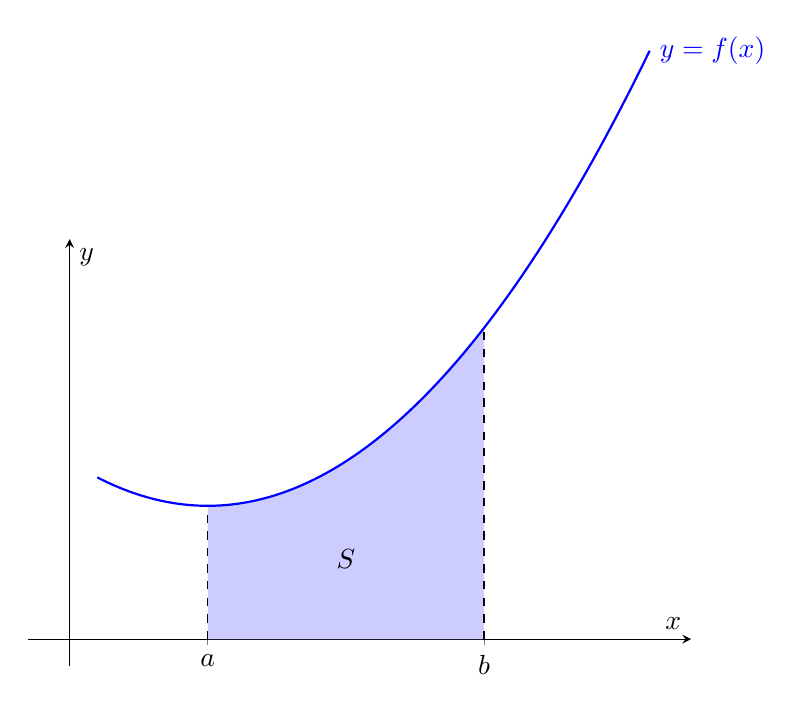
\begin{tikzpicture}
\begin{axis}[
    axis lines=middle,
    xlabel={$x$},
    ylabel={$y$},
    xmin=-0.3, xmax=4.5,
    ymin=-0.3, ymax=4.5,
    xtick={1,3},
    xticklabels={$a$,$b$},
    ytick=\empty,
    width=10cm, height=7cm,
    clip=false
]
% Fill the area under the curve
\addplot[fill=blue!20, draw=none, domain=1:3, samples=100] 
    {0.5*x^2 - x + 2} \closedcycle;
% Plot the curve
\addplot[thick, blue, domain=0.2:4.2, samples=100] 
    {0.5*x^2 - x + 2} node[right] {$y = f(x)$};
% Labels
\node at (axis cs:2, 0.9) {$S$};
\draw[dashed] (axis cs:1,0) -- (axis cs:1,{0.5*1^2 - 1 + 2});
\draw[dashed] (axis cs:3,0) -- (axis cs:3,{0.5*3^2 - 3 + 2});
\end{axis}
\end{tikzpicture}
\end{center}

\textbf{Bendresnis atvejis.} Kai funkcija $f(x)$ įgyja ir neigiamų reikšmių:
\begin{itemize}
    \item Ten, kur $f(x) > 0$, integralas skaičiuojamas su pliusu (plotas virš $Ox$ ašies).
    \item Ten, kur $f(x) < 0$, integralas skaičiuojamas su minusu (plotas po $Ox$ ašimi).
\end{itemize}

Todėl, norint rasti \textbf{geometrinį plotą} (neatsižvelgiant į ženklą), naudojama formulė:
\[
S = \int_a^b |f(x)|\,dx.
\]

Jei funkcija $f(x) \leq 0$ visoje atkarpoje $[a,b]$, plotas skaičiuojamas:
\[
S = -\int_a^b f(x)\,dx.
\]

\textbf{Dviejų kreivių apriboto ploto skaičiavimas.} Jeigu figūra apribota dviem kreivėmis 
$y = f(x)$ ir $y = g(x)$, kur $f(x) \geq g(x)$ atkarpoje $[a,b]$, tai jos plotas:
\[
S = \int_a^b \bigl[f(x) - g(x)\bigr]\,dx.
\]

\begin{example}
Apskaičiuokime plotą figūros, apribotos parabolės $y = x^2$ ir tiesės $y = x$.

\textit{Sprendimas.} Pirmiausia randame susikirtimo taškus: $x^2 = x \Rightarrow x(x-1) = 0$, 
taigi $x_1 = 0$, $x_2 = 1$. Atkarpoje $[0,1]$ teisinga $x \geq x^2$, todėl:
\[
S = \int_0^1 (x - x^2)\,dx = \left[\frac{x^2}{2} - \frac{x^3}{3}\right]_0^1 
  = \frac{1}{2} - \frac{1}{3} = \frac{1}{6}.
\]
Atsakymas: $S = \dfrac{1}{6}$ (plotas. vnt.$^2$).
\end{example}

%--------------------------------------------------------------------
\subsection{Niutono–Leibnico formulė}
%--------------------------------------------------------------------

Niutono–Leibnico formulė yra pagrindinis teorinis ir praktinis įrankis apibrėžtajam integralui 
apskaičiuoti. Ji sieja apibrėžtąjį integralą su pirmykšte funkcija.

\begin{theorem}[Niutono–Leibnico formulė]
Jeigu funkcija $f(x)$ yra tolydi atkarpoje $[a,\,b]$ ir $F(x)$ yra bet kuri jos pirmykštė 
funkcija, t.\,y. $F'(x) = f(x)$, tai:
\[
\boxed{\int_a^b f(x)\,dx = F(b) - F(a).}
\]
\end{theorem}

Įprastai rašoma trumpiau, naudojant dvitaškio žymėjimą:
\[
\int_a^b f(x)\,dx = \Big[F(x)\Big]_a^b = F(b) - F(a).
\]

\begin{remark}
Pirmykštės funkcijos $F(x)$ pasirinkimas neturi įtakos galutiniam rezultatui: jeigu 
$F_1(x) = F(x) + C$, tai $F_1(b) - F_1(a) = F(b) + C - F(a) - C = F(b) - F(a)$. 
Todėl integruojant pagal Niutono–Leibnico formulę konstanta $C$ nepridedama.
\end{remark}

\textbf{Skaičiavimo algoritmas:}
\begin{enumerate}
    \item Randame pointegralinės funkcijos $f(x)$ pirmykštę funkciją $F(x)$.
    \item Apskaičiuojame $F(b)$ ir $F(a)$.
    \item Randame skirtumą $F(b) - F(a)$.
\end{enumerate}

\begin{example}
Apskaičiuokite $\displaystyle\int_1^3 (2x + 1)\,dx$.

\textit{Sprendimas.}
\[
\int_1^3 (2x+1)\,dx = \Big[x^2 + x\Big]_1^3 = (9 + 3) - (1 + 1) = 12 - 2 = 10.
\]
\end{example}

\begin{example}
Apskaičiuokite $\displaystyle\int_0^{\pi} \sin x\,dx$.

\textit{Sprendimas.} Pirmykštė funkcija: $F(x) = -\cos x$.
\[
\int_0^{\pi} \sin x\,dx = \Big[-\cos x\Big]_0^{\pi} = (-\cos\pi) - (-\cos 0) = 1 + 1 = 2.
\]
\end{example}

\begin{example}
Apskaičiuokite $\displaystyle\int_1^{e} \frac{1}{x}\,dx$.

\textit{Sprendimas.} Pirmykštė funkcija: $F(x) = \ln x$.
\[
\int_1^{e} \frac{1}{x}\,dx = \Big[\ln x\Big]_1^{e} = \ln e - \ln 1 = 1 - 0 = 1.
\]
\end{example}

\subsubsection{Dažniausiai naudojamos formulės}

Žemiau pateikiama apibrėžtųjų integralų skaičiavimui naudingų pirmykščių funkcijų lentelė:

\renewcommand{\arraystretch}{1.8}
\begin{center}
\begin{tabular}{|c|c|}
\hline
\textbf{Funkcija} $f(x)$ & \textbf{Pirmykštė} $F(x)$ \\
\hline
$x^n$ $(n \neq -1)$ & $\dfrac{x^{n+1}}{n+1}$ \\
\hline
$\dfrac{1}{x}$ & $\ln|x|$ \\
\hline
$e^x$ & $e^x$ \\
\hline
$a^x$ & $\dfrac{a^x}{\ln a}$ \\
\hline
$\sin x$ & $-\cos x$ \\
\hline
$\cos x$ & $\sin x$ \\
\hline
$\dfrac{1}{\cos^2 x}$ & $\tg\, x$ \\
\hline
$\dfrac{1}{\sin^2 x}$ & $-\ctg\, x$ \\
\hline
\end{tabular}
\end{center}

\subsubsection{Apibrėžtojo integralo savybės}

Šios savybės dažnai praverčia sudėtingesniuose uždaviniuose:

\begin{enumerate}
    \item \textbf{Linijinumas:}
    \[
    \int_a^b \bigl[\alpha f(x) \pm \beta g(x)\bigr]\,dx 
    = \alpha\int_a^b f(x)\,dx \pm \beta\int_a^b g(x)\,dx,
    \quad \alpha, \beta \in \mathbb{R}.
    \]
    \item \textbf{Adityvinumas (intervalo dalijimas):}
    \[
    \int_a^b f(x)\,dx = \int_a^c f(x)\,dx + \int_c^b f(x)\,dx, \quad a < c < b.
    \]
    \item \textbf{Rėžių keitimas:}
    \[
    \int_a^b f(x)\,dx = -\int_b^a f(x)\,dx.
    \]
    \item \textbf{Lygybė:}
    \[
    \int_a^a f(x)\,dx = 0.
    \]
    \item \textbf{Nelygybė:} jei $f(x) \geq g(x)$ atkarpoje $[a,b]$, tai
    \[
    \int_a^b f(x)\,dx \geq \int_a^b g(x)\,dx.
    \]
\end{enumerate}

\begin{exercise}
Apskaičiuokite šiuos integralus naudodami Niutono–Leibnico formulę:
\begin{enumerate}[label=\alph*)]
    \item $\displaystyle\int_0^2 (3x^2 - 2x + 5)\,dx$
    \item $\displaystyle\int_1^4 \sqrt{x}\,dx$
    \item $\displaystyle\int_0^{\pi/2} \cos x\,dx$
    \item $\displaystyle\int_1^{e^2} \frac{2}{x}\,dx$
    \item $\displaystyle\int_{-1}^{1} (x^3 - x)\,dx$
\end{enumerate}
\end{exercise}

\begin{exercise}
Apskaičiuokite figūros, apribotos kreivės $y = x^2 - 4$ ir $Ox$ ašies, plotą.

\textit{Užuomina:} Pirmiausia raskite susikirtimo taškus su $Ox$ ašimi, 
tada apskaičiuokite $\displaystyle\int_a^b |f(x)|\,dx$.
\end{exercise}


\section{Integralų taikymai}

Apibrėžtinis integralas yra vienas galingiausių matematinių įrankių, leidžiančių tiksliai skaičiuoti geometrines charakteristikas – plotus ir tūrius. Šiame skyriuje nagrinėsime du pagrindinius taikymus, kurie dažnai sutinkami valstybinio brandos egzamino užduotyse.

% ─────────────────────────────────────────────
\subsection{Ploto skaičiavimas}
% ─────────────────────────────────────────────

\subsubsection{Kreivlinės trapecijos plotas}

\begin{definition}
\textbf{Kreivlinė trapecija} – tai figūra, kurią riboja funkcijos $y = f(x)$ grafikas, $Ox$ ašis ir tiesės $x = a$ bei $x = b$.
\end{definition}

Jeigu $f(x) \geq 0$ intervale $[a, b]$, kreivlinės trapecijos plotas apskaičiuojamas formule:
\[
S = \int_a^b f(x)\, dx
\]

Jeigu $f(x) \leq 0$ visame intervale $[a, b]$, tai integralas yra neigiamas, todėl plotą skaičiuojame:
\[
S = -\int_a^b f(x)\, dx = \int_a^b |f(x)|\, dx
\]

Bendrasis atvejis – kai funkcija keičia ženklą intervale $[a, b]$. Tuomet randame visus taškus $c_1, c_2, \ldots, c_k \in (a, b)$, kuriuose $f(c_i) = 0$, ir skaičiuojame:
\[
S = \int_a^b |f(x)|\, dx = \int_a^{c_1} |f(x)|\, dx + \int_{c_1}^{c_2} |f(x)|\, dx + \cdots + \int_{c_k}^{b} |f(x)|\, dx
\]

\begin{remark}
Egzamine dažna klaida – neskaičiuoti modulio ir tiesiog paimti galutinį integralą nuo $a$ iki $b$. Atsiminkite: plotas \textbf{visada} yra teigiamas dydis.
\end{remark}

\begin{example}
Apskaičiuokite figūros, apribotos funkcijos $f(x) = x^2 - 4$ grafiku ir $Ox$ ašimi, plotą.

\textbf{Sprendimas.} Randame funkcijos nulines vietas:
\[
x^2 - 4 = 0 \implies x = -2 \text{ arba } x = 2
\]
Intervale $[-2, 2]$ funkcija yra neigiama ($f(x) \leq 0$), todėl:
\[
S = -\int_{-2}^{2}(x^2 - 4)\, dx = -\left[\frac{x^3}{3} - 4x\right]_{-2}^{2}
\]
\[
= -\left[\left(\frac{8}{3} - 8\right) - \left(\frac{-8}{3} + 8\right)\right] = -\left[\frac{8}{3} - 8 + \frac{8}{3} - 8\right]
= -\left[\frac{16}{3} - 16\right] = 16 - \frac{16}{3} = \frac{32}{3}
\]
\textbf{Atsakymas:} $S = \dfrac{32}{3} \approx 10{,}67$ (ploto vienetai).
\end{example}

\subsubsection{Plotas tarp dviejų kreivių}

Jeigu dvi funkcijos $f(x)$ ir $g(x)$ yra tolydžios intervale $[a, b]$ ir $f(x) \geq g(x)$ visame šiame intervale, tai figūros, apribotos šių funkcijų grafikais, plotas:

\[
\boxed{S = \int_a^b \bigl[f(x) - g(x)\bigr]\, dx}
\]

čia $f(x)$ – viršutinė kreivė, $g(x)$ – apatinė kreivė.

\begin{remark}
Jeigu kreivės susikerta, reikia rasti susikirtimo taškus ir skaidyti integralą į dalis, kiekvienoje iš kurių aiškiai žinome, kuri kreivė yra aukščiau.
\end{remark}

\textbf{Algoritmas ploto tarp dviejų kreivių skaičiavimui:}
\begin{enumerate}
    \item Rasti $f(x)$ ir $g(x)$ susikirtimo taškus ($f(x) = g(x)$) – tai reiškia integravimo ribas $a$ ir $b$.
    \item Patikrinti, kuri funkcija yra didesnė intervale $(a, b)$ (pvz., pasirinkti vidinį tašką).
    \item Integruoti skirtumą $f(x) - g(x)$ (arba $g(x) - f(x)$) nuo $a$ iki $b$.
\end{enumerate}

\begin{example}
Apskaičiuokite figūros, apribotos parabolės $y = x^2$ ir tiesės $y = x + 2$, plotą.

\textbf{Sprendimas.}

\textbf{1 žingsnis.} Randame susikirtimo taškus:
\[
x^2 = x + 2 \implies x^2 - x - 2 = 0 \implies (x-2)(x+1) = 0
\]
Taigi $x_1 = -1$, $x_2 = 2$.

\textbf{2 žingsnis.} Intervale $[-1, 2]$ tiesiog patikriname: kai $x = 0$, $g(0) = 2 > f(0) = 0$, todėl $g(x) = x + 2 \geq f(x) = x^2$.

\textbf{3 žingsnis.}
\[
S = \int_{-1}^{2}\bigl[(x+2) - x^2\bigr]\, dx = \left[\frac{x^2}{2} + 2x - \frac{x^3}{3}\right]_{-1}^{2}
\]
\[
= \left(2 + 4 - \frac{8}{3}\right) - \left(\frac{1}{2} - 2 + \frac{1}{3}\right)
= \frac{10}{3} - \left(-\frac{7}{6}\right) = \frac{10}{3} + \frac{7}{6} = \frac{20}{6} + \frac{7}{6} = \frac{27}{6} = \frac{9}{2}
\]
\textbf{Atsakymas:} $S = \dfrac{9}{2} = 4{,}5$ (ploto vienetai).
\end{example}

\begin{exercise}
Apskaičiuokite figūros, apribotos funkcijų $f(x) = \sqrt{x}$ ir $g(x) = x^2$, grafikais, plotą.
\end{exercise}

\begin{exercise}
Raskite figūros, kurią riboja $y = \sin x$ ir $Ox$ ašis intervale $[0, 2\pi]$, plotą.
\end{exercise}


% ─────────────────────────────────────────────
\subsection{Tūrio skaičiavimas}
% ─────────────────────────────────────────────

\subsubsection{Sukimosi kūno tūris}

Kai kreivlinė trapecija, apribota funkcijos $y = f(x) \geq 0$ grafiku ir $Ox$ ašimi intervale $[a, b]$, sukama aplink $Ox$ ašį, susidaro \textbf{sukimosi kūnas}.

\begin{definition}
\textbf{Sukimosi kūnas} – tai erdvinis kūnas, gaunamas sukant plokštuminę figūrą aplink tam tikrą ašį.
\end{definition}

\subsubsection{Diskų metodas}

Sukimosi kūną galime įsivaizduoti kaip begalybę plonausiųjų diskų, kurių spindulys $r = f(x)$ ir storis $dx$. Vieno disko tūris:
\[
dV = \pi \cdot [f(x)]^2 \cdot dx
\]

Susumuję visus diskus gauname:
\[
\boxed{V = \pi \int_a^b [f(x)]^2\, dx}
\]

\begin{example}
Apskaičiuokite tūrį kūno, gauto sukant $y = \sqrt{x}$ aplink $Ox$ ašį intervale $[0, 4]$.

\textbf{Sprendimas.}
\[
V = \pi \int_0^4 (\sqrt{x})^2\, dx = \pi \int_0^4 x\, dx = \pi \left[\frac{x^2}{2}\right]_0^4 = \pi \cdot \frac{16}{2} = 8\pi
\]
\textbf{Atsakymas:} $V = 8\pi \approx 25{,}13$ (tūrio vienetai).
\end{example}

\begin{example}
Apskaičiuokite sferos, kurios spindulys $R$, tūrį naudodami integralą.

\textbf{Sprendimas.} Sfera gaunama sukant pusapskritimį $y = \sqrt{R^2 - x^2}$ aplink $Ox$ ašį nuo $-R$ iki $R$:
\[
V = \pi \int_{-R}^{R} \bigl(\sqrt{R^2 - x^2}\bigr)^2\, dx = \pi \int_{-R}^{R} (R^2 - x^2)\, dx
\]
\[
= \pi \left[R^2 x - \frac{x^3}{3}\right]_{-R}^{R} = \pi \left[\left(R^3 - \frac{R^3}{3}\right) - \left(-R^3 + \frac{R^3}{3}\right)\right]
= \pi \cdot \frac{4R^3}{3} = \frac{4}{3}\pi R^3
\]
Taip integralais išvedama klasikinė sferos tūrio formulė $V = \dfrac{4}{3}\pi R^3$.
\end{example}

\subsubsection{Žiedo (poveržlės) metodas}

Jeigu sukamas plotas tarp dviejų funkcijų $f(x) \geq g(x) \geq 0$ intervale $[a, b]$, kūno skerspjūvis yra žiedas. Žiedo plotas:
\[
A(x) = \pi \bigl[f(x)\bigr]^2 - \pi \bigl[g(x)\bigr]^2
\]

Todėl tūris:
\[
\boxed{V = \pi \int_a^b \Bigl([f(x)]^2 - [g(x)]^2\Bigr)\, dx}
\]

\begin{example}
Apskaičiuokite tūrį kūno, gauto sukant plotą tarp $y = x$ ir $y = x^2$ (intervale $[0,1]$) aplink $Ox$ ašį.

\textbf{Sprendimas.} Intervale $[0,1]$ turime $x \geq x^2$, todėl $f(x) = x$, $g(x) = x^2$:
\[
V = \pi \int_0^1 \bigl(x^2 - x^4\bigr)\, dx = \pi \left[\frac{x^3}{3} - \frac{x^5}{5}\right]_0^1 = \pi\left(\frac{1}{3} - \frac{1}{5}\right) = \pi \cdot \frac{2}{15} = \frac{2\pi}{15}
\]
\textbf{Atsakymas:} $V = \dfrac{2\pi}{15} \approx 0{,}42$ (tūrio vienetai).
\end{example}

\subsubsection{Formulių apžvalga}

\begin{tcolorbox}[title={Pagrindinės integralų taikymo formulės}, colback=blue!5!white, colframe=blue!60!black]
\begin{center}
\renewcommand{\arraystretch}{2}
\begin{tabular}{|l|c|}
\hline
\textbf{Uždavinys} & \textbf{Formulė} \\
\hline
Plotas po $f(x)$ grafiku & $\displaystyle S = \int_a^b f(x)\, dx$ \quad ($f(x) \geq 0$) \\
\hline
Plotas, kai $f(x)$ keičia ženklą & $\displaystyle S = \int_a^b |f(x)|\, dx$ \\
\hline
Plotas tarp dviejų kreivių & $\displaystyle S = \int_a^b [f(x) - g(x)]\, dx$ \quad ($f \geq g$) \\
\hline
Tūris (diskų metodas) & $\displaystyle V = \pi \int_a^b [f(x)]^2\, dx$ \\
\hline
Tūris (žiedo metodas) & $\displaystyle V = \pi \int_a^b \left([f(x)]^2 - [g(x)]^2\right)\, dx$ \\
\hline
\end{tabular}
\end{center}
\end{tcolorbox}

\begin{exercise}
Apskaičiuokite tūrį kūno, gauto sukant figūrą, apribotą $y = x^2 + 1$ ir $y = 0$ intervale $[0, 2]$, aplink $Ox$ ašį.
\end{exercise}

\begin{exercise}
Apskaičiuokite kūgio, kurio pagrindo spindulys $r$ ir aukštis $h$, tūrį, sukant tiesę $y = \dfrac{r}{h}x$ aplink $Ox$ ašį nuo $0$ iki $h$.
\end{exercise}

